\input{/Users/daniel/github/config/preamble.sty}%This is available at github.com/danimalabares/config

%\usepackage[style=authortitle-terse,backend=bibtex]{biblatex}
%\addbibresource{bibliography.bib}

\begin{document}

\begin{minipage}{\textwidth}
	\begin{minipage}{1\textwidth}
		Geometria Simpl\'etica \hfill Daniel González Casanova Azuela
		
		{\small Profs. Henrique Bursztyn e Leonardo Macarini\hfill\href{https://github.com/danimalabares/sg}{github.com/danimalabares/sg}}
	\end{minipage}
\end{minipage}\vspace{.2cm}\hrule

\vspace{10pt}
{\huge Lista 5}

\tableofcontents

\addcontentsline{toc}{section}{Problem 1}
\begin{idea1}{Problem 1}\leavevmode
	Let  $G$ be a Lie group. Let $X:G\longrightarrow TG$ be a section of the projection $TG\longrightarrow G$, not necessarily smooth. Show that if  $X$ is left invariant (i.e., $dL_g(X)=X\circ L_g$ for all $g\in G$), then $X$ is automatically smooth.

	Conclude that an analogous result holds for differential forms: if a section $\eta:G\to \Lambda^{k}(T^*G)$ is left-invariant ($L^*_g\eta=\eta$), then $\eta$ is a smooth $k$-form. Check that an analogous result holds for $G$-invariant forms on a homogeneous manifold.
\end{idea1}

\begin{proof}[Solution]\leavevmode
	(Idea by my) We know that $X_g=dL_g(X_e)$. We want to show that the map $G \to TG:g\mapsto dL_g(X_e)$ is smooth. Suggestion by Ted Shiffrin is to consider 
	\begin{align*}
		\mu: G\times G &\longrightarrow G \\
		(g,h) &\longmapsto L_gh=gh
	\end{align*}
	which is smooth and thus has smooth differential which turns out to have the expression
	\begin{align*}
		d\mu: TG\times TG &\longrightarrow TG \\
		(u_g,v_h) &\longmapsto dR_hu_g+dL_g v_h
	\end{align*}
	Choosing $g$ arbitrary, $h=e$, $u_g=0$ and $v_h=X_e$, we obtain
	\[d\mu(u_g,v_h)=dL_gX_e\]
	and, as we have said, this differential depends smoothly on $g$.

	To generalize this result we just notice that left multiplication $L_g$ induces smooth maps the Grassman algebra by
	\begin{align*}
		\mathbf{L_g}: \Lambda^{k}(G) &\longrightarrow \Lambda^{k}(G) \\
		\eta &\longmapsto \begin{aligned}
			\mathbf{L_g}\eta: \mathfrak{X}^k(G) &\longrightarrow \mathbb{R} \\
			(X_1,\ldots,X_k) &\longmapsto (dL_gX_1,\ldots,dL_gX_1)
		\end{aligned}
	\end{align*}
and similarly group multiplication $\mu$ induces maps
\begin{align*}
	\mu: \Lambda^{k}(G) \times \Lambda^{k}(G)&\longrightarrow \Lambda^{k}(G) \\
	(\alpha,\beta) &\longmapsto \mathbf{R_h}\alpha+\mathbf{L_g}\beta
\end{align*}
so again chosing 
	
\end{proof}

\addcontentsline{toc}{section}{Problem 2}
\begin{idea4}{Problem 2}\leavevmode
	\begin{enumerate}[label=\alph*.]
		\item Prove that any connected Lie group $G$ is generated as a group by any open neighbourhood $U$ of the identity element (i.e. $G=\bigcup_{n=1}^\infty U^n$).
		\item Suppose that two Lie group homomorphisms $\varphi,\psi:G\to H$ are such that $d\varphi|_{e}=d\psi|_{e}$. Show that $\varphi$ and $\psi$ coincide on the connected component of $G$ containing the identity $e$.
	\end{enumerate}
\end{idea4}

\addcontentsline{toc}{section}{Problem 3}
\begin{idea1}{Problem 3}\leavevmode
	Consider the Lie groups $\mathsf{SU}(2) =\{A\in\mathcal{M}_{2}(\mathbb{C})|AA^*=\operatorname{Id}, \det A=1\}$ and $\mathsf{SO}(3) =\{A\in\mathcal{M}_{3}(\mathbb{R})|AA^{\mathbf{T}}=\operatorname{Id},\det A=1\}$.
	\begin{enumerate}[label=\alph*.]
		\item Show that
		\[\mathsf{SU}(2) =\left\{ \begin{pmatrix} a&b\\-\bar{b}&\bar{a} \end{pmatrix} ,a,b\in\mathbb{C},|a|^2+|b|^2=1\right\} \]
		Conclude that, as a manifold $\mathsf{SU}(2)$ is diffeomorphic to $S^3$ (hence it is simply connected).

		Recall the definition of the quaternions $\mathbb{H}$. Show that the sphere $S^3$, seen as quaternions of norm 1, inherits a Lie group structure with respect to which it is isomorphic to $\mathsf{SU}(2)$.

	\item Verify that
		\begin{equation}\label{eq:1}
			\mathfrak{su}(2) =\left\{ \begin{pmatrix} i\alpha &\beta\\-\bar{\beta} &-i\alpha \end{pmatrix} ,\alpha\in\mathbb{R},\beta\in\mathbb{C} \right\} .
		\end{equation}
		Consider the identification $\mathfrak{su}(2) \cong \mathbb{R}^{3}$, that takes the element in $\mathfrak{su}(2)$ determined by $\alpha,\beta$ to the vector $(\alpha,\operatorname{Re}\beta,\operatorname{Im}\beta)$ in $\mathbb{R}^{3}$. Observe that, with respect to this identification, $ \det $ in $\mathfrak{su}(2)$ corresponds to $\|\cdot\|^2$ in $\mathbb{R}^{3}$.


	\item Verify that each element $A\in\mathsf{SU}(2)$ defines a linear transformation on the vector space $\mathfrak{su}(2)$ by conjugation: $B\mapsto ABA^{-1}$. Show that, with the identification $\mathfrak{su}(2) \cong \mathbb{R}^{3}$, we obtain a representation (i.e., a linear action) of $\mathsf{SU}(2)$ on $\mathbb{R}^{3}$ that is norm preserving. Conclude that we have homomorphism $\phi:\mathsf{SU}(2) \to \mathsf{O}(3)$, verifying that is image is $\mathsf{SO}(3)$ and its kernel is $\{\operatorname{Id},-\operatorname{Id}\}$.

	\item Conclude that $\mathsf{SU}(2) \cong S^3$ is a double cover of $\mathsf{SO}(3)$ *hence is its universal cover, since it's simply connected), qnd the covering map identifies antipodal points of $S^3$. Hence, as manifolds, $\mathsf{SO}(3)$ is identified with $\mathbb{R}P^{3}$.
	\end{enumerate}
\end{idea1}

\begin{proof}[Solution]\leavevmode
	\begin{enumerate}[label=\alph*.]
		\item Given the computation {\color{2}above}, it is clear that $\mathsf{SU}(2)$ is diffeomorphic to $S^3$ since its parameters $a,b\in\mathbb{C}$, $|a|^2+|b|^2=1$, can be understood as vectors $x\in\mathbb{R}^{4}$ of norm 1.

		The quaternions are the only 4-dimensional real division algebra. This means it is a 4-dimensional real vector space equipped with a (non-commutative) multiplication. They are also equipped with a norm that coincides with euclidean norm. With respect to this norm we define the unit sphere $S^3$. 
		
			To see that $S^3$ is a Lie subgroup we first need to check that it is closed under quaternion product. The easiest way to see that is via quaternion conjugate: if $x=x_1+ix_2+jx_3+kx_4$ is a quaternion, its conjugate is $\bar{x}=x_1-ix_2-jx_3-kx_4$. It may be computed that the norm is given by $|x| =x\bar{x}$. Then we see that if $x,y\in S^3$
			\[|xy\overline{xy}|=|xy\bar{y}\bar{x}| =\Big|x|y| \bar{x}\Big|=1\]
			Then the fact that $S^3$ is a Lie group follows from the fact that the restricition (the multiplication and inverse map) of smooth maps to embedded submanifolds remains smooth (\cite{lee}, prop ?).

			An identification between $S^3\subset \mathbb{H}$ and $\mathsf{SU}(2)$ as expressed above is given by
			\[a+bi+cj+dk\longmapsto \begin{pmatrix} a+bi&c+di\\-c+di&a-bi\end{pmatrix} \]
			Checking that this map is a group isomorphism ammounts to checking that matrix multiplication in $\mathsf{SU}(2)$ is the same as quaternion multiplication 


			\item (Proof from \cite{hall}, prop. 3.24 and coro. 3.46).
				\begin{enumerate}[label=\textbf{Step \arabic*}]
					\item Show that the tangent space at identity of a matrix Lie group $G$ (definition in lectures) is the same as the matrices $X$ such that $ \operatorname{exp}(tX) \in G$ for all $t\in\mathbb{R}$.

						\begin{proof}[Proof of Step 1]\leavevmode
							(\cite{hall}, coro. 3.46) If $X \in T_{\operatorname{Id}}G$, by definition of exponential map we have $\operatorname{exp}(tX) \in G$.%Define a curve $\gamma$ via the exponential map (seen in lectures, also see figure): $\gamma(t)=\operatorname{exp}(tX)$ which is in $G$ by definition of exponential map.
	\begin{figure}[H]		\centering
		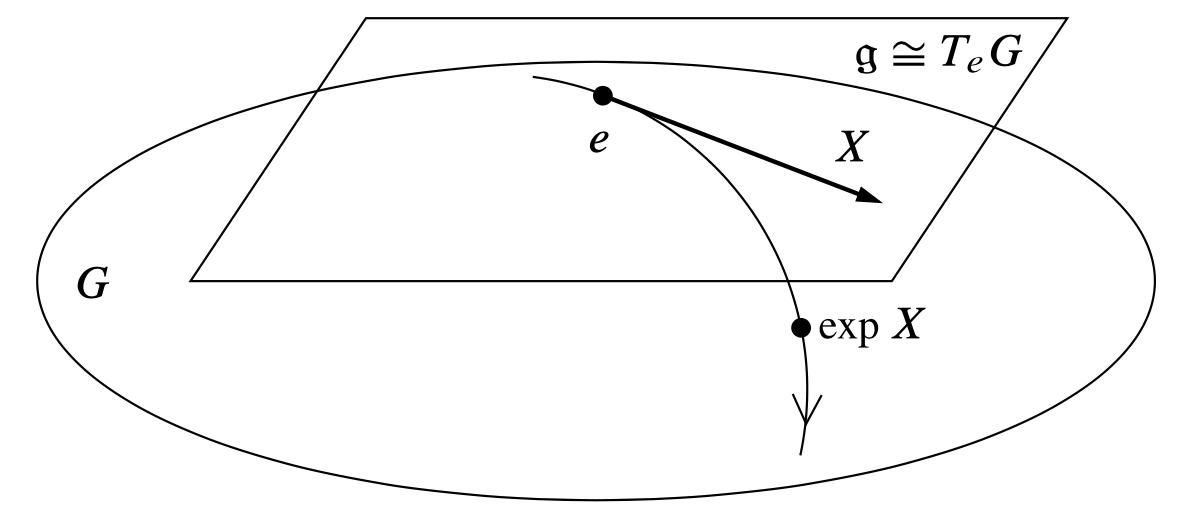
\includegraphics[width=0.4\textwidth]{fig2}	
	\caption*{\cite{lee}, fig. ?}\end{figure}
Now suppose that $X$ is such that $\operatorname{exp}(tX)\in G$ for all $t\in\mathbb{R}$.

	I got stuck with the proof in Hall so I will use prop 20.3 from \cite{lee}. The idea is to show see $\mathsf{SU}(2)$ as a subgroup of, say $\mathsf{GL}(2,\mathbb{C})$. Then a
						\end{proof}

					\item Then we look for the matrices such that for all $t\in\mathbb{R}$,
						\[\operatorname{exp}(tX)^* =(\operatorname{exp}(tX)^{-1}=\operatorname{exp}(-tX) \qquad \text{ and} \qquad \det \operatorname{exp}(tX)=1. \]
						This means that
						\[\operatorname{exp}(tX^*) =\operatorname{exp}(-tX) \qquad \text{and} \qquad \operatorname{ Tr}(X)=0.\]
						The first condition is equivalent to $X^*=-X$. Thus we see that
						\[\mathfrak{su}(2)=\{X\in\mathcal{M}_{2\times 2}(\mathbb{C}):X^* =-X\text{ and }\operatorname{Tr}(X)=0 \}\]
		
					\item It is immediate that the expression in \cref{eq:1} is contained in the set above. For the other inclusion first notice that the condition $X^*=-X$ makes the entries in the diagonal be such that
						\begin{align*}							x+iy&=-\overline{x+iy}=-(x-iy)=-x+iy\implies x=-x\implies x=0						\end{align*}
						while the traceless condition implies the two entries in the diagonal must be additive inverses. For the entries in the antidiagonal we literally see the definition of conjugate transpose.
				\end{enumerate}

Now let's identify $\mathfrak{su}(2)$ with $\mathbb{R}^{3}$ via $\alpha,\beta \mapsto (\alpha,\operatorname{Re}\beta,\operatorname{Im}\beta)$. We immediately see that
\[\det \begin{pmatrix} i\alpha&\beta\\-\bar{\beta} &-i\alpha\end{pmatrix} =i\alpha(-i\alpha)=\beta(-\bar{\beta} )=\alpha^2+|\beta|^2=\|(\alpha,\operatorname{Re}\beta,\operatorname{Im}\beta)\|^2\]

\item De acordo como exercício anterior, é suficiente mostrar que $ABA^{-1}$ tem traza zero é $ABA^{-1}=-(ABA^{-1})^*$. A primeira propriedade é imediata dado que, em geral, $\operatorname{Tr}(XY)=\operatorname{Tr}(YX)$. Para a segunda propriedade note que
	\[(ABA^{-1})^*=(A^{-1})^*B^*A^*=(A^*)^*(-B)A^{-1}=-ABA^{-1}\]
	O fato de que essa ação em $\mathsf{SU}(2)$ preserva a norma é immediato do item anterior e do fato de que determinante de um produto de matrizes é o produto dos determinantes.

	Isso significa que cada elemento em $\mathsf{SU}(2)$ é uma transformação linear $\mathbb{R}^{3}\to \mathbb{R}^{3}$, i.e. um mapa $\mathsf{SU}(2)\to \mathsf{O}(3)$. Esse mapa é um homomorfismo já que 
\end{enumerate}
\end{proof}

\addcontentsline{toc}{section}{Problem 4}
\begin{idea4}{Problem 4}\leavevmode
	Let $\mathfrak{g}$ be the Lie algebra of a Lie group $G$, and let  $k:\mathfrak{g} \times \mathfrak{g}\to \mathbb{R}$be a symmetric bilinear form that is $\operatorname{Ad}$-invariant (i.e. $k(\operatorname{Ad}_g(u),\operatorname{Ad}_g(v))=k(u,v)$ for $g\in G$).
	\begin{enumerate}[label=\alph*.]
		\item Show that the map
			\begin{equation}\label{Eq:4a}\begin{aligned}
				k^\sharp:\mathfrak{g}  &\longrightarrow \mathfrak{g}^* \\
				k^\sharp(u)(v) &=k(u,v)\end{aligned}
			\end{equation}
			is $G$-equivariant:
			\[k^\sharp \circ \operatorname{Ad}_g=(\operatorname{Ad}^*)_g\circ k^\sharp,\qquad \forall g\in G\]
			[\textit{Recall:} $(\operatorname{Ad}^* )_g:=(\operatorname{Ad}_{g^{-1}})^*$.] In particular, when $k$ is nondegenerate (i.e. $k^\sharp$ is an isomorphism), the adjoint and coadjoint actions are equivalent.

		\item Verify that \cref{Eq:4a} implies that $k([w,u],v)=-k(u,[w,v])$,  $\forall u,v,w\in\mathfrak{g}$, and that both conditions are equivalent when $G$ is connected.
	\end{enumerate}
\end{idea4}

\begin{proof}[Solução]
	\begin{enumerate}[label=\alph*.]
		\item É só abrir as definições . Fixe um elemento $x\in\mathfrak{g}$. No lado esquerdo, temos
			\[k^\sharp \circ \operatorname{Ad}_g(x)=k^\sharp(\operatorname{Ad}_gx)=k(\operatorname{Ad}_gx,\cdot )\]
			e no lado direito,
			\[(\operatorname{Ad}^* )_g\circ k^\sharp (x)=\operatorname{Ad}^*_g(k^\sharp (x))=\operatorname{Ad}^* _g(k(x,\cdot ))=k(x,\operatorname{Ad}_{g^{-1}}\cdot )\]
			mas, como $k$ é $\operatorname{Ad}$-invariante,
			$k(x,\operatorname{Ad}_{g^{-1}},\cdot )=k(\operatorname{Ad}_gx,\cdot )$.

		\item Must check this later…
	\end{enumerate}
\end{proof}

\addcontentsline{toc}{section}{Problem 5}
\begin{idea1}{Problem 5}\leavevmode
For a Lie algebra $\mathfrak{g}$, there is always a canonical bilinear form $k:\mathfrak{g} \times \mathfrak{g} \to \mathbb{R}$, called \textit{\textbf{Killing form}}, given by:
\[k(u,v)=\operatorname{tr}(\operatorname{ad}_u\operatorname{ad}_v).\]
(\textit{Recall:} $\operatorname{ad}_u:\mathfrak{g} \to \mathfrak{g}$, $\operatorname{ad}_u(v)=[u,v]$.)
\begin{enumerate}[label=\alph*.]
	\item Note that $k$ is symmetric, and check that it is  $\operatorname{Ad}$-invariant.
	\item A Lie algebra is called \textit{\textbf{semi-simple}} if $k$ is nondegenerate. Show that $\mathfrak{so}(3)$ is semi-simple.
\end{enumerate}
\end{idea1}

\begin{proof}[Solution]\leavevmode
	\begin{enumerate}[label=\alph*.]
		\item O fato de $k$ ser simétrica segue de que, em geral, $\operatorname{tr}(AB)=\operatorname{tr}(BA)$. Para ver que $k$ é $\operatorname{Ad}$-invariante, note que, para $g\in G$,
			\begin{align*}
				k(\operatorname{Ad}_gu,\operatorname{Ad}_gv)&=\operatorname{tr}(\operatorname{ad}_{\operatorname{Ad}u}\operatorname{ad}_{\operatorname{Ad}v})= \operatorname{tr}([\operatorname{Ad}u,[\operatorname{Ad}v,\cdot ]])=
			\end{align*}
	\end{enumerate}
\end{proof}

\addcontentsline{toc}{section}{Problem 6}
\begin{idea4}{Problem 6}\leavevmode
	Consider the linear isomorphism $\mathbb{R}^{3}\to \mathfrak{so}(3)$, given by
	\[v=(x,y,z)\longmapsto \hat{v}:=\begin{pmatrix} 0&-z&y\\z&0&-x\\-y&x&0 \end{pmatrix} \]
	\begin{enumerate}[label=\alph*.]
		\item Describe the Lie bracket on $\mathbb{R}^{3}$ induced by the commutator in $\mathfrak{so}(3)$, and the inner product in $\mathfrak{so}(3)$ that corresponds to the canonical inner product in $\mathbb{R}^{3}$.

		\item Describe the $\mathsf{SO}(3)$-action on $\mathbb{R}^{3}$ corresponding to the adjoint action, its orbits, as well as its infinitesimal generators. Find (without any calculation!) a description of the coadjoint action on $\mathbb{R}^{3}$ (identified with $(\mathbb{R}^{3})^*$ through the canonical inner product).
	\end{enumerate}
\end{idea4}

\begin{proof}[Solution]\leavevmode
	\begin{enumerate}[label=\alph*.]
		\item Lembre que
			\[\mathsf{SO}(3) =\{A\in\mathcal{M}_{3}(\mathbb{R}):A A^{\mathbf{T}}=\operatorname{Id},\det A=1\}\]
			\[\mathfrak{so}(3) =\{A\in\mathcal{M}_{3}(\mathbb{R}):A=-A^{\mathbf{T}}\}\]
Isso explica por que as matrizes em $\mathfrak{so}(3)$ tem a forma mostrada acima. O isomorfismo com $\mathbb{R}^{3}$ é dado por
	\begin{align*}
		 \mathfrak{so}(3) &\longrightarrow \mathbb{R}^{3} \\
		\begin{pmatrix} 0&-z&y\\z&0&-x\\-y&x&0 \end{pmatrix}  &\longmapsto \begin{pmatrix} x\\y\\z \end{pmatrix} =u\\
		[U,V ]& \longmapsto u\times v\\
		\frac{1}{2}\operatorname{tr}(UV^{\mathbf{T}})&\longmapsto\left<u,v\right> 
	\end{align*}
Para comprovar que de fato o commutador de $\mathfrak{so}(3)$ corresponde com o produto vetorial em $\mathbb{R}^{3}$, considere duas matrizes $U,V\in\mathfrak{so}(3)$ e os vetores correspondentes $u=(u_1,u_2,u_3)$, $v=(v_1,v_2,v_3)$. O commutador é
\begin{align*}
	[U,V]=UV-VU&=\begin{pmatrix} 0&-u_3&u_2\\u_3&0&-u_1\\-u_2&u_1&0 \end{pmatrix} \begin{pmatrix} 0&-v_3&v_2\\v_3&0&-v_1\\-v_2&v_1&0 \end{pmatrix} \\
	&- \begin{pmatrix} 0&-v_3&v_2\\v_3&0&-v_1\\-v_2&v_1&0 \end{pmatrix} 
\begin{pmatrix} 0&-u_3&u_2\\u_3&0&-u_1\\-u_2&u_1&0 \end{pmatrix}\end{align*}
	\end{enumerate}
	a entrada $(3,2)$ da matriz resultante  é a primeira coordenada do vetor correspondente a $[U,V]$; esse numero é claramente $u_1v_3-u_3v_2$. Analogamente, a segunda coordenada é $u_3v_1-u_1v_3$, enquanto a terceira $u_1v_2-u_2v_1$. Essas são as coordenadas de $u\times v$.

Para ver que o produto interno de $\mathbb{R}^{3}$ corresponde com $\frac{1}{2}\operatorname{tr}$ note que
\begin{align*}
	UV^{\mathbf{T}}=U(-V)&=\begin{pmatrix} 0&-u_3&u_2\\u_3&0&-u_1\\-u_2&u_1&0 \end{pmatrix} \begin{pmatrix} 0&v_3&-v_2\\-v_3&0&v_1\\v_2&-v_1&0 \end{pmatrix} \\
		       &=\begin{pmatrix} u_3v_3+u_2v_2&*&*\\ *&u_3v_3+u_1v_1&*\\ *&*&u_2v_2+u_1v_1 \end{pmatrix} 
\end{align*}

Agora vamos calcular a ação coadjunta. 
Primeiro notemos que a ação coadjunta, definida como a derivada do operador $I_A(X)=AXA^{-1}$, é ela mesma. Talvez esse é um fato obvio porque $I_A$  é um mapa linear, e a sua derivada coincide com ele. Porém, tem um argumento mais explícito no \href{https://math.stackexchange.com/questions/512026/prove-that-the-action-of-a-lie-group-on-its-lie-algebra-via-the-adjoint-represen}{StackExchange}: a ação adjunta em um vetor  $X\in\mathfrak{so}(3)$ que seja a derivada em $t=0$ da curva $c\subset \mathsf{SO}(3)$, i.e.  $c'(0)=X$, é simplesmente $\frac{d}{dt}Ac(t)A^{-1}\Big|_{t=0}=AXA^{-1}$. A observação chave é que como a álgebra de Lie $\mathfrak{so}(3)$ é um álgebra de matrizes, o produto do lado direito está bem definido.

Em fim, agora vou seguir \href{https://www.ethaneade.org/lie.pdf}{este documento} para achar uma matriz que representa esse operador linear cuando identificamos $\mathfrak{so}(3)$ com $\mathbb{R}^{3}$. Mais precisamente, queremos achar uma matriz  $\overline{\operatorname{Ad}_A}$ tal que $\operatorname{Ad}_AX=AXA^{-1}\rightsquigarrow \overline{\operatorname{Ad}_A}x$ onde $x\in\mathbb{R}^{3}$  representa a matriz $X\in\mathfrak{so}(3)$.

O truque é usar que as matrizes em $\mathsf{SO}(3)$, sendo isometrías de $\mathbb{R}^{3}$, preservam o produto vetorial, i.e. $Ax\times Ay=A(x \times y)$ para qualquer $x,y\in\mathbb{R}^{3}$. Temos que
\begin{align*}
	\operatorname{Ad}_AXAy&=
\end{align*}
\end{proof}

\addcontentsline{toc}{section}{Problem 7}
\begin{idea1}{Problem 7}\leavevmode
	Let $(V,\Omega)$ be a symplectic vector space, and consider $H:=V\times \mathbb{R}=\{(v,t)\}$. This space $H$ with the multiplication
	\[(v_1,t_1)\cdot(v_2,t_2)=\left( v_1+v_2,\frac{1}{2}\Omega(v_1,v_2)+t_1+t_2 \right) \]
	is a Lie group called the \textit{\textbf{Heisenberg group}} (find the identity elements and inverses in  $H$).
	\begin{enumerate}[label=\alph*.]
		\item Show (directly from the conjugation formula in $H$) that $\operatorname{Ad}_{(v,t)}(X,r)=(X,r+\Omega(v,X))$, for $(X,r)\in\mathfrak{h}=\mathsf{Lie}(H) =V\times \mathbb{R}$. Describe the adjoint orbits, verifying that their possible dimensions are zero and one.
		\item Verify that $\operatorname{ad}_{(Y,s)}(X,r)=(0,\Omega(Y,X))$. [Recalling that $\operatorname{ad}_{(Y,s)}(X,r)=[(Y,s),(X,r)]$, we obtain a formula for the Lie bracket in $ \mathfrak{h}$.]
		\item Describe the coadjoint action of $H$ on $\mathfrak{h}^*=V^*\times \mathbb{R}^*$ and its orbits, analyzing the possible dimensions.
	\end{enumerate}
\end{idea1}

\begin{proof}[Solution]\leavevmode
É imediato que a identidade em $H$ é $(0,0)\in V\times \mathbb{R}$, e o elemento inverso de $(v,t)$  é $(-v,-t)$.
 \begin{enumerate}[label=\alph*.]
	\item Primeiro note que $\operatorname{Ad}_{(v,t)}X=(v,t)\cdot X\cdot(-v,-t)$ onde $\cdot$ denota o produto en $H\cong \mathfrak{h}$ (esse isomorfismo é claro já que $H$ é um espaço vetorial, assim o espaço tangente em $(0,0)$  é isomofo a ele). Para justificar isso (como no exercício anterior), considere uma curva $\gamma\subset H$ tal que $\gamma(0)=(0,0)$ e $\gamma'(0)=(X,r)$. Então 
		\begin{align*}
			\operatorname{Ad}_{(v,t)}(X,r)&=d_{(0,0)}I_{(v,t)}(X,r)=\frac{d}{d\tau}I_{(v,t)}\circ \gamma\Big|_{\tau=0}\\&=\frac{d}{d\tau}(v,t)\cdot \gamma(\tau)\cdot(-v,-t)\Big|_{\tau=0}=(v,t)\cdot (X,r)\cdot(-v,-t).
		\end{align*}
daí é só calcular
		\begin{align*}
			\operatorname{Ad}_{(v,t)}(X,r)&=(v,t)\cdot(X,r)\cdot(-v,-t)\\
			&=(v,t)\cdot\left(X-v, \frac{1}{2}\Omega(X-r)+r-t \right) \\
			&=\left( X,\frac{1}{2}\Omega(v,X-v)+t+\frac{1}{2}\Omega(X,-v)+r-t \right) \\
			&=\left( X,\frac{1}{2}\Omega(v,X)+\frac{1}{2}\Omega(v,-v)+\frac{1}{2}\Omega(X,-v)+s \right) \\
			&=(X,\Omega(v,X)+r)
		\end{align*}
A órbita adjunta de $(X,r)$  é $X\times \mathbb{R}$ sempre que $X\neq 0$ já que $\Omega$ é não degenerada. Caso $X=0$, a  órbita é um ponto, $(0,r)$.

\item 

\end{enumerate}
\end{proof}
\end{document}
